\documentclass[8.5pt,twoside,twocolumn]{article}
\oddsidemargin -1.2cm
\evensidemargin -1.2cm
\textwidth 18cm
\headheight 1.0in
\topmargin -3.5cm
\textheight 22cm
\usepackage[super,sort&compress,comma]{natbib}
\usepackage{amsmath}
%\usepackage{mhchem}
\usepackage{times,mathptmx}
% \usepackage{times}
% feel free not to use mathptmx if it causes difficulties
\usepackage{sectsty}
\usepackage{balance} 

\usepackage{graphicx} %eps figures can be used instead
\usepackage{lastpage}
\usepackage[format=plain,justification=raggedright,singlelinecheck=false,font=small,labelfont=bf,labelsep=space]{caption} 
\usepackage{fancyhdr}
\pagestyle{fancy}

\usepackage{SIunits}
\DeclareMathOperator{\erf}{erf}

\begin{document}

\thispagestyle{plain}
\fancypagestyle{plain}{
\fancyhead[L]{
\includegraphics[height=8pt]{headers/LH}}
\fancyhead[C]{\hspace{-1cm}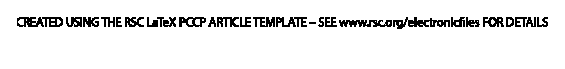
\includegraphics[height=20pt]{headers/CH}}
\fancyhead[R]{
\includegraphics[height=10pt]{headers/RH}\vspace{-0.2cm}}
\renewcommand{\headrulewidth}{1pt}}
\renewcommand{\thefootnote}{\fnsymbol{footnote}}
\renewcommand\footnoterule{\vspace*{1pt}% 
\hrule width 3.4in height 0.4pt \vspace*{5pt}} 
\setcounter{secnumdepth}{5}



\makeatletter 
\def\subsubsection{\@startsection{subsubsection}{3}{10pt}{-1.25ex plus -1ex minus -.1ex}{0ex plus 0ex}{\normalsize\bf}} 
\def\paragraph{\@startsection{paragraph}{4}{10pt}{-1.25ex plus -1ex minus -.1ex}{0ex plus 0ex}{\normalsize\textit}} 
\renewcommand\@biblabel[1]{#1}            
\renewcommand\@makefntext[1]% 
{\noindent\makebox[0pt][r]{\@thefnmark\,}#1}
\makeatother 
\renewcommand{\figurename}{\small{Fig.}~}
\sectionfont{\large}
\subsectionfont{\normalsize} 

\fancyfoot{}
\fancyfoot[LO,RE]{\vspace{-7pt}
\includegraphics[height=9pt]{headers/LF}}
\fancyfoot[CO]{\vspace{-7.2pt}\hspace{12.2cm}
\includegraphics{headers/RF}}
\fancyfoot[CE]{\vspace{-7.5pt}\hspace{-13.5cm}
\includegraphics{headers/RF}}
\fancyfoot[RO]{\footnotesize{\sffamily{1--\pageref{LastPage} ~\textbar  \hspace{2pt}\thepage}}}
\fancyfoot[LE]{\footnotesize{\sffamily{\thepage~\textbar\hspace{3.45cm} 1--\pageref{LastPage}}}}
\fancyhead{}
\renewcommand{\headrulewidth}{1pt} 
\renewcommand{\footrulewidth}{1pt}
\setlength{\arrayrulewidth}{1pt}
\setlength{\columnsep}{6.5mm}
\setlength\bibsep{1pt}

\twocolumn[
  \begin{@twocolumnfalse}
\noindent\LARGE{\textbf{Particle-level size determination and its influence on the ordering of supercooled hard sphere colloids}}
\vspace{0.6cm}

\noindent\large{\textbf{Mathieu Leocmach\textit{$^{a}$} and
Hajime Tanaka$^{\ast}$\textit{$^{a}$}}}\vspace{0.5cm}
%Please note that \ast indicates the corresponding author(s) but no footnote text is required. 


\noindent\textit{\small{\textbf{Received Xth XXXXXXXXXX 20XX, Accepted Xth XXXXXXXXX 20XX\newline
First published on the web Xth XXXXXXXXXX 200X}}}

\noindent \textbf{\small{DOI: 10.1039/b000000x}}
\vspace{0.6cm}
%Please do not change this text.

\noindent \normalsize{We propose a scale-space based method to extract both the individual 3D coordinates and the radii of spherical colloids from confocal microscopy images. According to synthetic and real data, dilute or crowded, particles can be detected correctly without assumption on their sizes, even when particle diameters differ by large factors. Moreover the size of each particle can be estimated within a few percent error (less than $0.3\%$ if the diameter is larger than \unit{5}{px}).}
\vspace{0.5cm}
 \end{@twocolumnfalse}
  ]
\title{Particle-level size determination and its influence on the ordering of supercooled hard sphere colloids.}

\footnotetext{\textit{$^{a}$~Institute of Industrial Science, University of Tokyo, 4-6-1 Komaba, Meguro-ku, Tokyo 153-8505, Japan. E-mail: tanaka@iis.u-tokyo.ac.jp}}

%\author{Mathieu Leocmach} 

%\author{Hajime Tanaka}
%\affiliation{ {Institute of Industrial Science, University of Tokyo, 4-6-1 Komaba, Meguro-ku, Tokyo 153-8505, Japan} }

%\date{Received \today}

\section*{Introduction}

Experimental physicists often need to recognize objects, count them, follow them and characterise them. \citet{perrin} had to count colloids by hand to establish the sedimentation-diffusion equilibrium. Nowadays computer vision algorithms are used routinely in the lab to track hundreds of thousands of objects as diverse as stars in a galaxy~\cite{Bertin1996}, tracers in a microfluidic device~\cite{Wereley2010}, dust in a plasma or viruses in a living cell~\cite{Brandenburg2007}. In all these cases, tracking is possible if the particles are either point-like and far apart, or several pixel wide and almost monodisperse in size. To our knowledge, algorithm that allow tracking of polydisperse particles in crowded environments have not reached the softmatter community.

Overall size distribution influences crystallisation~\cite{Pusey1987,Henderson1996,Fasolo2003,Schope2007,pusey2009hard}, glass forming ability~\cite{Pusey1987,Henderson1996,Senkov2001,Schope2007,pusey2009hard}, sedimentation~\cite{Binks1998,Leocmach2010} and emulsion stability~\cite{Biben1993,Binks1998} among other physical phenomena. It can be characterized by various methods that rely on measurements done in well-controlled environments~\cite{Lange1995,Provder1997,Finder2004}. However the local size distribution is not accessible experimentally in situ and is thus not studied.

Particle-level microscopy experiments usually access the coordinates of the particles via the algorithm proposed by \citet{Crocker1996}. The original noisy image is blurred by convolution with a Gaussian kernel of width $\sigma$ to yield a soft peak per particle. Local intensity maxima within this blurred image give the coordinates of the particles with pixel resolution. Sub-pixel resolution ($0.1\sim0.3$~pixels error) can be achieved by taking the centre of mass of a neighbourhood around the local maxima. The extension of this algorithm to localize particles in 3D confocal microscopy images has been done in two ways: either tracking particles in each confocal plane and reconstructing the results (2D-flavour)~\citep{vanblaaderen1995rss, Lu2007}, or full image analysis on three dimensional pictures (3D-flavour)~\citep{dinsmore2001tdc}.

The choice of the width $\sigma$ of the blurring kernel is critical: if it is too small, then the intensity profile is flat near the centre  of a particle, leading to multiple and ill-localized maxima per particle; if it is too large, then the peaks of nearby particles overlap, leading to shifts in the detected positions, or even fusion of the particles (only one particle detected instead of two). If the colloids are fairly monodisperse one can argue (at least in the 3D-flavour) that there exists a range of possible width where the choice of $\sigma$ has almost no effect on the number of particles detected. Choosing $\sigma$ within this range gives confidence in the localisation results.

\begin{figure*}
\centering
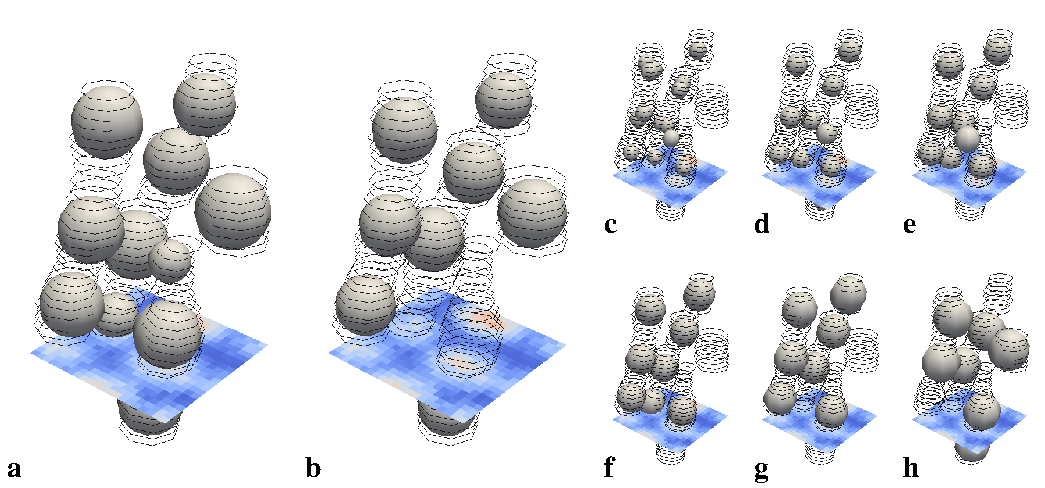
\includegraphics{fig_localise.pdf}
\caption{\textbf{Visualisation of the results of various tracking methods for the same portion of image.} \textbf{a,} Multiscale 3D tracking. \textbf{b,} Reconstruction from multiscale 2D tracking. \textbf{c-h,} Crocker and Grier in 3D with blurring radius increasing from \unit{2}{px} to \unit{4.5}{px} by steps of \unit{0.5}{px}. The circles on each picture are the result of 2D multiscale tracking of each XY slice of the 3D pictures. Sphere are displayed with radii determined by the tracking methods in \textbf{a-b}, and equal to the blurring radius for \textbf{c-h}.}
	\label{fig:localise}
\end{figure*}

However, we found that no such ``good blur width'' exists in a sample of moderate ($6-7\%$) polydispersity (see Fig.~\ref{fig:localise}c-h). The detection of smaller particles with small blurring is incompatible with the detection of the larger particles, and conversely. This unacceptable failure of the \citet{Crocker1996} algorithm, as well as the want of the particles' radii data, triggered our design of a novel localisation algorithm that would be robust even for a system of any finite polydispersity, which is unavoidable and sometime desired in real experiments.

The key notion to detect objects of unknown and possibly diverse sizes in an image is the \emph{scale space}~\cite{Lindeberg1993}. A popular implementation for isotropic objects (or ``blobs'') is the Scale Invariant Feature Transform (\textsc{sift}) of \citet{Lowe2004}. It is often used to match between different images from complex objects consisting of many rigidly linked blobs (e.g. to create a large scale image from overlapping pictures)~\citep{Lowe2004, Urschler2006, Cheung2009}. To our knowledge, this method was never used for the quantitative localisation and sizing of independent single-blob objects like spherical colloids, droplets in an emulsion or crystal nuclei.

In the following part, we will describe our localisation method and its results on synthetic but more and more realistic data. In the second part of the paper, we will focus on the specific case of 3D confocal data. In the third part we will apply our method to a supercooled liquid of polydisperse hard spheres observed by confocal microscopy and extract local polydispersity. Finally in the last part we will show more briefly other applications that we deem useful for the soft matter and microfluidics communities, including 2D data of wide field fluorescent microscopy and phase contrast microscopy.

\section*{Localisation and sizing method}

\begin{figure*}
\centering
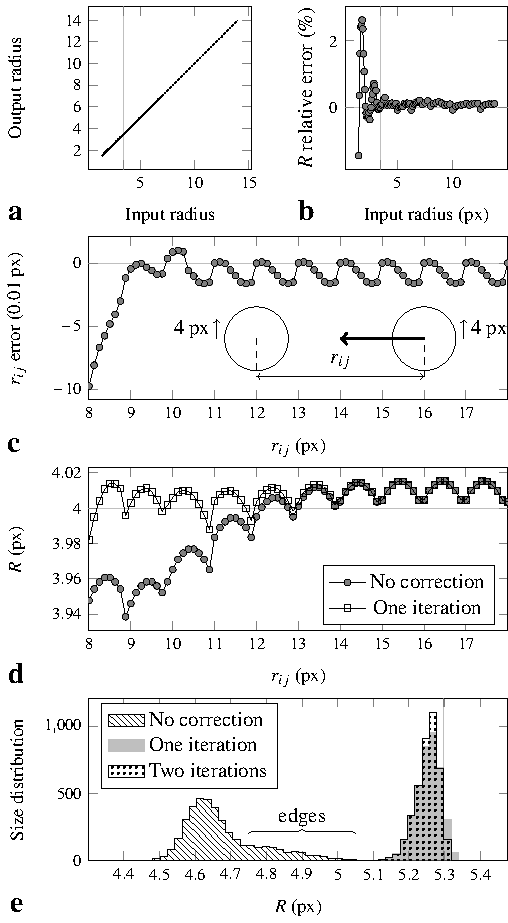
\includegraphics{fig_perfect.pdf}
	\caption{\textbf{Results from perfect images.} \textbf{a} Sizing of an isolated sphere. Left of the vertical line our algorithm uses a doubled image. \textbf{b} Localisation error and \textbf{c} sizing error function of the distance between two particles. Oscillations are due to off-lattice centre position. \textbf{d} Size distribution extracted from digitized configuration of 4000 monodisperse hard spheres at $0.50$ volume fraction (the vertical line indicates the input radius). The tail to the right is due to particles on the edges of the image who have fewer neighbours and thus are more `dilute'. \textbf{c} and \textbf{d} also show the effect of finite dilution correction up to convergence.}
	\label{fig:perfect}
\end{figure*}

In this section, we will start by recalling the principle of \textsc{sift}, then we will explain our method in the ideal case of an isolated binary ball, to add successively finite dilution and difference in brightness between the particles. Here we assume perfect noiseless, distortion-free, images. The objects to localise are thus (pixellised) balls of uniform intensity. To mimic the low resolution of experimental images in our test images (see Fig.~\ref{fig:perfect}), we draw uniformly white balls on a 4 to 16 times larger image and then we reduce accordingly the resolution using area resampling.

\subsection*{Scale invariant feature transform}
The \textsc{sift} consists in convolving the original image $I$ by Gaussian kernels $g_{\sigma_s}$ of logarithmically increasing widths $\sigma_s$ to obtain a series of blurred images $G_s$
\begin{align}
\forall s>0,\quad G_s = I \star g_{\sigma_s}, \label{eq:gaussian_blur}\\
\intertext{where $\star$ is the convolution operator and}
\forall s>0,\quad \sigma_{s} = 2^{s/n} \sigma_0 ,
\label{eq:sigma_s}
\end{align}
with $n$ a fixed integer. Following \cite{Lowe2004} we use $\sigma_0=1.6$ and $n=3$. Bright objects in the original image appear as bright blobs in the blurred images, and the blobs fuse together as the kernel width increases. This can be seen as a lower and lower-pass filter in the frequency domain. If we take the difference between consecutive blurred images we obtain a comb of band pass filtered versions of $I$: 
\begin{equation}
\forall s>1,\quad DoG_s = G_s - G_{s-1} \label{eq:DoG_s}
\end{equation}
The difference of Gaussians (DoG) response function defined in this way depends on the position in space and on the scale. Bright objects in the original image are detected as local minima in $DoG_s$. Furthermore, the intensity of the response is optimal at a $\sigma$ that can be related to the size of the object (see below). Thus a local minima in both space and scale in the response function DoG indicates both localisation and \emph{size} of an object, without any assumption on the target size.

As in the case of the \citet{Crocker1996} algorithm, the \textsc{sift} can be extended in three dimensions in two ways: either by extracting 2D blobs independently on each slice and then reconstructing 3D objects (Fig.~\ref{fig:localise}b) or by working directly in three dimensions~\cite{Urschler2006, Cheung2009} (Fig.~\ref{fig:localise}a). We found that the former method is prone to errors, missing about a tenth of the particles in our best implementation (Fig.~\ref{fig:localise}b). The 3D results presented in this paper are obtained solely by the later method.

We stress that a volumetric implementation of \textsc{sift} implies a large amount of data (typically more than \unit{1}{\giga b} for a $(\unit{256}{px})^3$ picture) and thus requires careful memory management.

\subsection*{Sub-pixel and sub-scale resolution}
The DoG constructed above is defined on a $d+1$ dimensional grid, with $d$ the spatial dimensionality. One can interpolate it as a continuous function of the position $\vec{r}$ and the scale $s$ and thus localise the minima with a precision below the grid size, which corresponds to sub-pixel resolution on the position and sub-scale sizing~\citep{Lowe2004}. We found that second order estimate of the spatial derivatives and first order estimates of the scale derivatives gave the best precision.

The object-by-object optimal scale determination allows us to perform the spatial sub-pixel resolution step for each object on an image that is blurred just enough to have neither a flat intensity profile nor affected by the overlap with a nearby object's blob. We found that if for a given object the DoG is minimum at $\sigma_s$, the best image to use is $G_{s-1}$. This leads to a spatial resolution below $0.1$~pixels when two $8$-pixels wide particles are at hard-core contact, and less than $0.02$~pixels error ($0.3\%$ of the diameter) when any other particle's surface is further than $1$~pixel from the surface of the particle of interest (see Fig.~\ref{fig:perfect}b).

\subsection*{Sizing at infinite dilution}

The analytical response of a binary ball to a Gaussian blur, at the centre of the ball is a function of dimensionless ratio $x=R/\sqrt{2}\sigma$: $G(x)$ (see Appendix~\ref{sec:gaussian_vs_ball} for an exact expression). The DoG response function is the difference between the two such functions. However, the choice of the width of the two functions is not arbitrary: we make the difference between two consecutive blurred images, the image blurred by $\sigma_{j+1}$ and the image blurred by $\sigma_j$. Therefore, in each of our discrete DoG images the value at the centre of the particle can be expressed as
\begin{align}
DoG(R,\sigma_j, \alpha) = DoG(x_j, \alpha) &= G(x_j/\alpha) - G(x_j),\\
\intertext{with $\alpha=2^{1/n}$. Given sub-scale refinement, this can be written as a continuous function of $\sigma$:}
DoG(R,\sigma, \alpha) = DoG(x, \alpha) &= G(x/\alpha) - G(x).
\end{align}

Here it is clear that minimizing $DoG(x, \alpha)$ with respect to $x$ yields a value $x^*$ that depends only on $\alpha$. Exact calculation yields:
\begin{equation}
	x^* = R/\sqrt{2}\sigma^* = \sqrt{\frac{3\ln \alpha}{1-\alpha^{-2}}}, 
	\label{eq:scale_dil}
\end{equation}
Practically one obtains $\sigma^*$, the value of $\sigma$ that minimises $DoG(R,\sigma, \alpha)$, by a polynomial fit for discrete data $\sigma_j$. Eq.~(\ref{eq:scale_dil}) allows to translate the $n$-dependent $\sigma^*$ to the parameter-free real radius of the particle, $R$. The error on $R$ does depend on the number of subdivisions. We found that with $n=3$ the radius of an isolated pixelated ball can be indeed measured within $0.3\%$ relative error with this method (see Fig.~\ref{fig:perfect}a).

The scale $s=0.5$ corresponds (via Eq.~(\ref{eq:sigma_s}) and Eq.~(\ref{eq:scale_dil})) to the smaller detectable radius $R_{min}\approx \unit{3.5}{px}$ ($\sigma_0=1.6$, $n=3$). In order to detect small objects, \citet{Lowe2004} recommends to double the size of the input image using linear interpolation prior to building the first level of the pyramid. This method fares relatively well in noiseless images (see Fig.~\ref{fig:perfect}a) despite larger errors, but we found that it has to be use with care in confocal images due to noise and deconvolution artefacts. In addition doubling image size implies a 8-fold increase in memory consumption (reaching \unit{60}{\giga b} in the case of a $(\unit{512}{px})^3$ original image). Our implementation allows this on $\unit{64}{byte}$ computers by relying on memory mapped files, nevertheless it is mostly impractical. All following tests results are obtained without relying on doubled images.

\subsection*{Edge and overlap removal}

The difference-of-Gaussian function has a strong response not only at the center of bright objects but also along their edges. To eliminate these spurious detections, \citet{Lowe2004} suggests to construct the local Hessian matrix around each minimum of the DoG and then compare its eigenvalues to identify elongated objects.

We found that this was often not enough, especially in crowded environments where an isolated void induces local minima of the DoG response with rather isotropic signatures on the edge of nearby particles. An other case not covered by the Hessian technique is the physically hierarchical structure of many softmatter systems, e.g. particles forming clusters. In this situation our algorithm detects a blob for each particle and a much larger blob for the cluster. In both cases the DoG response of the spurious feature is smaller (less negative) than the one of the valid particles covering the same portion of space. Using the above radius, we looked for pairs of particles closer to each other than the larger of their radii. This means the centre of one of the particles is situated inside the other. In the physical systems we study, this cannot be correct due to excluded volume effects, thus we remove the feature of lesser DoG response. One may be tempted to implement a hard core exclusion (no pair of particle closer than the sum of their radii) to eliminate even more spurious detection. We found that the gain was extremely limited ($0.01\%$ of the detected features suppressed) and that imprecision in positioning or in sizing caused valid particles to be discarded.

We note that the orientation of non-spherical particles or the deformation of soft objects can be monitored in principle by using the local Hessian matrix.

\subsection*{Finite dilution}
The Gaussian (and DoG) response of a particle decays rapidly away from its surface (see Eq.~(\ref{eq:split_G}). We found that even at contact the position shift induced by a nearby particle was less than a tenth of a pixel (see Fig.~\ref{fig:perfect}b). However when two particles are closer than a few times the blurring width, their influence on each other cannot be neglected: the minima of the DoG is effectively shifted toward smaller scales, leading to smaller radii if one uses Eq.~(\ref{eq:scale_dil}) out of the dilute context (see Fig.~\ref{fig:perfect}c).

The response of $N$ particles of radii $\lbrace R_i\rbrace$ can be superimposed at any scale $\sigma$ and at any point of space, in particular we define $DoG_i$ as the response at the centre of particle $i$.
\begin{equation}
%\forall i,\quad 
DoG_i(\lbrace A_j\rbrace, \lbrace r_{ij}\rbrace, \lbrace R_j\rbrace, \sigma) = \sum_j A_j DoG(r=r_{ij}, R=R_j, \sigma),
\label{eq:superpos}
\end{equation}
where the function $DoG(r,R,\sigma)$ is the response of a particle of radius $R$ at distance $r$ from its centre; $r_{ij}$ is the distances between particles $i$ and $j$ and $\lbrace A_i\rbrace$ are the respective brightness of the particles. The \textsc{sift} algorithm yields $\lbrace \sigma_i\rbrace$ so that for all $i$, $DoG_i$ is minimum with respect to $\sigma$ at $\sigma_i$, thus differentiating Eq.~(\ref{eq:superpos}) with respect to $\sigma$:
\begin{equation}
\forall i,\quad \frac{\partial DoG_i}{\partial\sigma}(\lbrace A_j\rbrace, \lbrace r_{ij}\rbrace, \lbrace R_j\rbrace, \sigma_i) = 0.
\label{eq:DoG_min}
\end{equation}

The system defined by Eq.~(\ref{eq:DoG_min}) is non linear with respect to $\lbrace R_j\rbrace$ but can be solved iteratively by Newton's method:
\begin{equation}
\left[ \frac{\partial^2 DoG_i}{\partial R_j\partial\sigma}\right] \times \left( \lbrace R_j\rbrace^{(k+1)} - \lbrace R_j\rbrace^{(k)} \right) = -\frac{\partial DoG_i}{\partial\sigma}
\label{eq:Newton}
\end{equation}
where the matrix and the right hand side are computed given $(\lbrace A_j\rbrace, \lbrace r_{ij}\rbrace, \sigma_i)$ and iteratively $\lbrace R_j\rbrace^{(k)}$, with the upper parenthesised index indicating the iteration rank. The results of Eq.~(\ref{eq:scale_dil}) are good starting values for the radii.

Using Eq.~(\ref{eq:superpos}), the elements of the matrix simplify to
\begin{equation}
\frac{\partial^2 DoG_i}{\partial R_j\partial\sigma} =  A_j \frac{\partial^2 DoG}{\partial R\partial\sigma}(r=r_{ij}, R=R_j^{(k)}, \sigma=\sigma_i)
\end{equation}

In principle Eq.~(\ref{eq:Newton}) is a $N\times N$ system of equations. However the DoG functions and its derivatives are rapidly decaying functions, thus the matrices are actually very sparse (about as many non-zero coefficients as particles in the first coordination shell), alleviating dramatically the computational burden when using sparse system solvers. Figure~\ref{fig:perfect}c shows the result of such correction for two identical particles, where Eq.~(\ref{eq:Newton}) converges in a single iteration. In many body case (see Fig.~\ref{fig:perfect}d) convergence is reached in two iterations. However the extremely low error of the dilute case is not totally recovered ($\approx 3\%$ relative error rather than $0.3\%$).

\subsection*{Brightnesses}

To solve Eq.~(\ref{eq:Newton}), one needs knowledge of the brightnesses $\lbrace A_i\rbrace$. In a first approximation, they can be assumed equal to a constant, which allow to simplify them out. This is often a sensible approximation. Nevertheless, the particles in an experimental image are not uniformly bright due to synthesis imperfection (quantity of dye fixed by each particle) and photo bleaching. If one does not take into account the relative brightness of the particles the less bright will appear smaller.

A better approximation is to measure during the \textsc{sift} process the value of the DoG response at the position and scale of each particle, \emph{i.e.} $DoG_i(\lbrace A_j\rbrace, \lbrace r_{ij}\rbrace, \lbrace R_j\rbrace, \sigma_i)$. Given the (iterative) values of the $\lbrace R_j\rbrace^{(k)}$, one can solve Eq.~(\ref{eq:superpos}) to get an iterative value of $\lbrace A_i\rbrace^{(k)}$. With respect to the brightnesses, Eq.~(\ref{eq:superpos}) is a linear system of $N$ equations with $N$ unknowns, thus directly solvable. It is also as sparse as Eq.~(\ref{eq:Newton}).

To sum up, the coefficients $\lbrace A_i\rbrace$ can be computed along with the radii in a joint iterative process:
\begin{enumerate}
\item Use Eq.~(\ref{eq:scale_dil}) to get the $\lbrace R_i\rbrace^{(0)}$
\item Solve the linear system given by Eq.~(\ref{eq:superpos}) to get the $\lbrace A_i\rbrace^{(k)}$ \label{it:A}
\item Solve the system given by Eq.~(\ref{eq:Newton}) to get the $\lbrace R_i\rbrace^{(k+1)}$ \label{it:R}
\item Iterate through steps \ref{it:A} and \ref{it:R} until convergence
\end{enumerate}


In our tests, we found that this algorithm converges as quickly with and without the brightness determination.

\section*{Confocal images}
\subsection*{Effect of a point spread function}
\begin{figure}
\centering
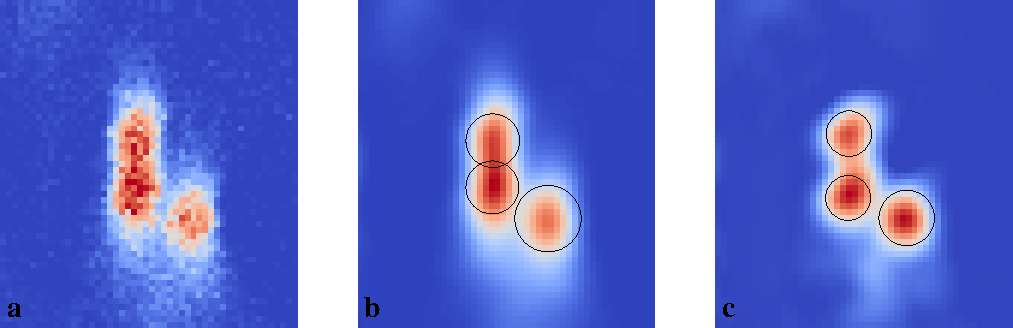
\includegraphics{fig_deconv.pdf}
	\caption{\textbf{Deconvolution.} Detail of the same $YZ$ slice of \textbf{a} original confocal image, \textbf{b} previous blurred by $\sigma_0=1.6$, \textbf{c} previous deconvolved by measured kernel. Circles indicate the tracked particles position and size when using whether \textbf{b} or \textbf{c} as first Gaussian layer $G_0$. All three centres are in the slice $\pm \unit{0.5}{px}$. \textbf{d} Radial distribution function of sticky spheres localised (blue) without and (red) with deconvolution.}
	\label{fig:deconv}
\end{figure}

Real images suffer from optical limitations, \emph{e.g.} the point-spread function (\textsc{psf}) of the microscope. In particular, spherical particles observed by confocal microscopy seem elongated along $Z$. The influence of such anisotropic distortion on the Gaussian and DoG responses is not trivial and most of the equations given in Appendix~\ref{sec:gaussian_vs_ball} do not have analytical equivalents. In particular, the minimum of the DoG response is found at larger values of $R/\sigma$, thus the naive use of the methods detailed in previous section lead to overestimate particle sizes.

In addition, the overlap of neighbouring particle images is no more negligible when the particles are aligned along $Z$. This leads to large imprecision in particle positions, especially in the case of anisotropic environment (e.g. isolated pair of particles, interface, gel). In Fig.~\ref{fig:deconv}d the radial distribution function of almost monodisperse colloids with short range attraction displays a shoulder before its first peak, indicating that particles centres are often found closer than the sum of their hard core radii, as illustrated in Fig.~\ref{fig:deconv}b.

We found that these issues were better addressed by pre-processing the images (as detailed below) rather than post processing the \textsc{sift} output \emph{via} analytical methods.

\subsection*{Deconvolution}
The image $y$ acquired by a microscope can be expressed as 
\begin{equation}
y = x \star h + \epsilon
\end{equation}
where $x$ is the perfect image, $h$ is the \textsc{psf} of the microscope and $\epsilon$ is the noise independent of both $x$ and $h$. The process of estimating $x$ from $y$ and some theoretical or measured expression of $h$ is called deconvolution. Deconvolution in presence of noise is a difficult problem~\cite{Riad1986}. Hopefully here we don't need to reconstruct the original image, but only our first Gaussian blurred version of it, \emph{i.e.} $G_0$. Indeed, after a reasonable amount of blur in three dimensions, the noise can be neglected and we obtain:
\begin{equation}
y_0 = (x \star h + \epsilon) \star g_{\sigma_0} \approx G_0 \star (h \star g_{\sigma_0})
\end{equation}
or in Fourier space
\begin{equation}
\mathcal{F}[y_0] = \mathcal{F}[G_0] \times \mathcal{F}[H]
\label{eq:Fourier_conv}
\end{equation}

Once $\mathcal{F}[H]$ is known the deconvolution reduces to a simple division in Fourier space. Let us measure $H$ in an isotropic system where we can write
\begin{align}
\left\langle \left|\mathcal{F}_X[G_0]\right|^2 \right\rangle  &= \left\langle \left|\mathcal{F}_Z[G_0]\right|^2 \right\rangle \\
\text{using Eq.~(\ref{eq:Fourier_conv})}\qquad 
\frac{\left\langle\left|\mathcal{F}_X[y_0]\right|^2 \right\rangle}{\left|\mathcal{F}_X[H]\right|^2}  &= \frac{\left\langle \left|\mathcal{F}_Z[y_0]\right|^2\right\rangle}{\left|\mathcal{F}_Z[H]\right|^2} \\
\intertext{In point scanning confocal imaging, the \textsc{psf} has negligible lobes along $X$ and $Y$ ($X$ only for line scanning), thus}
\left|\mathcal{F}_Z[H]\right|^2 &= \frac{\left\langle \left|\mathcal{F}_Z[y_0]\right|^2\right\rangle}{\left\langle\left|\mathcal{F}_X[y_0]\right|^2 \right\rangle}\\
\intertext{For example an Hermitian kernel (real valued spectrum)}
\mathcal{F}_Z[H] &= \sqrt{\frac{\left\langle \left|\mathcal{F}_Z[y_0]\right|^2\right\rangle}{\left\langle\left|\mathcal{F}_X[y_0]\right|^2 \right\rangle}}
\end{align}

Figure~\ref{fig:deconv}b-c shows the particles localized from the original image and from the deconvolved image. Deconvolution mends both size overestimation and imprecision in $z$ coordinate. This also translates in the radial distribution function (Fig.~\ref{fig:deconv}d), where the shoulder before the first peak disappears.

\subsection*{From optical to hard-core radius}

The method exposed above relies on the uniformity of the brightness within each particle to extract optical radii that is a good approximation to the physical (hard core) radii. However a colloidal particle often shows a smooth intensity profile under the microscope, less bright at the edge than at the center of the particle. This can be due to inhomogeneous fixation of the dye during the colloid synthesis, but the bottom line is the in-plane \textsc{psf} not corrected for in our above deconvolution method.

Under such conditions, the particles are detected smaller than their expected size. The real to optical size ratio has to be set using our knowledge of the sample. For example one may use the position of the first peak of the $g(r)$ to measure the average hard-core diameter. In general the real to optical size ratio may depends on the size of the particles and may evolve in time (i.e. because of photobleaching). We present below a detailed analysis of these issues for a case system.

We also note that darker edges lead to smaller influence of a particle on the DoG response of its neighbours. A smaller optical radius makes the particles optically further from each other. Accordingly, we found that finite dilution corrections were less important in real images than in our synthetic test images. For the same reason, the scaling factor must be applied after --- \emph{not} before --- finite dilution corrections.


\section*{Case study of a colloidal hard sphere supercooled liquid}

\subsection*{Experimental}
We used \textsc{pmma} (poly(methyl methacrylate)) colloids sterically stabilized with methacryloxypropyl terminated \textsc{pdms} (poly(dimethyl siloxane)) and fluorescently labelled with rhodamine isothiocyanate chemically bonded to the \textsc{pmma}. The colloids were suspended in a solvent mixture of cis-decalin and cyclohexyl-bromide for both optical index and density matching. To screen any (weak) electrostatic interactions, we dissolved tetrabutylammonium bromide salt, to a concentration of \unit{300}{\nano\mole\per\liter}~\citep{royall2005}. The estimated Debye screening length is \unit{13}{\nano\metre}, well below the length scale of the colloids that can be considered as hard spheres. The \unit{8}{bit} graylevel data was collected on a Leica SP5 confocal microscope, using \unit{532}{\nano\meter} laser excitation and voxel size of $(\unit{283}{\nano\metre})^2\times\unit{293}{\nano\metre}$.

\subsection*{Global polydispersity}

We localise the particles using our method, removed half-overlapping features and applied a single iteration of finite dilution corrections for both intensities and radii to obtain the optical radius of each particle. We then estimate the hard-core diameter function of the optical radius $R$ by locating the first peak of the partial radial distribution function $g_R(r)$ of the particles having $R_i$ close to $R$. As shown in Fig.~\ref{fig:sizing}a, the real to optical size ratio is around $1.5$ and is rather constant respective to $R$, thus a single overall scaling factor is enough. It can be determined by a single partial $g_R(r)$ with $R$ near the peak of the size distribution, or by locating the peak of $g(\hat{r})$. However, we found that this ratio was increasing with time due to photobleaching. We fit this increase by a linear relation and applied the resulting time-dependent ratio to obtain the real size of each particles.

\begin{figure}
\centering
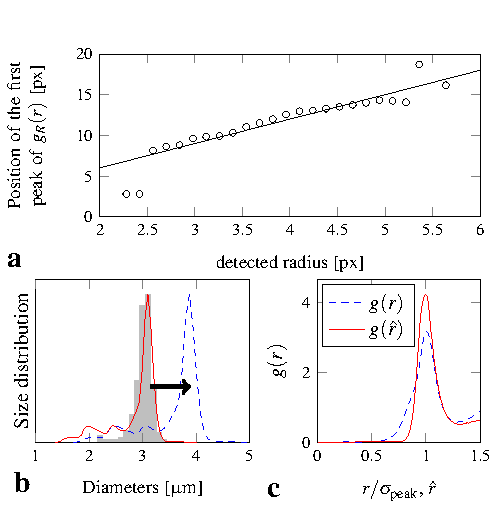
\includegraphics{fig_sizing.pdf}
	\caption{\textbf{\emph{In situ} sizing of colloids in a glass.} \textbf{a,} Position of the first peak of the partial $g_R(r)$ function of the optical radius $R$. Solid line corresponds to a real radius to optical radius ratio of $1.5$. \textbf{b,} Size distribution estimated \emph{in situ} (dashed line) by our multiscale algorithm ($\sim 10^7$ instantaneous sizing). Comparison with the size distribution estimated from \textsc{sem} of only $140$ dry particles (steps) is possible once $23\%$ of swelling of particle diameters is taken into account (full line). \textbf{c,} First peak of the radial distribution function with (full line) and without (dashed) the individual sizes data. Taking into account the measured sizes rectifies the effect of the polydispersity: the peak is thinner and higher.}
	\label{fig:sizing}
\end{figure}

Figure~\ref{fig:sizing}b shows the size distribution only $140$ dry colloids measured on high resolution scanning electron microscopy (\textsc{sem}) images. We also show the size distribution obtained by our \emph{in situ} measurements ($\sim 1.7\times 10^6$ instantaneous sizing in a $\approx 0.57$ volume fraction suspension). The later compares well with the former once a solvent swelling of $23\%$ in radius is taken into account. The polydispersity measured \emph{in situ} is $6.9\%$, where the polydispersity computed from \textsc{sem} is $6.2\%$.

The consistency of our method can be checked by constructing the radial distribution function $g(r)$. In monodisperse hard spheres, the $g(r)$ has a sharp first peak at $r=2R$ corresponding to hard core contact. Polydispersity implies hard core contacts at various $r$ and thus broadens the peak. One can recover a sharp peak by constructing $g(\hat{r})$, with $\hat{r}_{ij} = r_{ij}/(R_i+R_j)$. In Fig.~\ref{fig:sizing}c we successfully used the sizes measured by our method to rectify the first peak.

\subsection*{Polydispersity and structural heterogeneity}

\section*{Other applications}

\subsection*{Nucleation rate in a molecular liquid}

\subsection*{Tracking droplets in a microfluidic device}

Fluorescently labelled water-in-oil droplets obtained by standard microfluidic procedures~\cite{Montagne2011}

\section*{Conclusion}
Recently \citet{Kurita2011,Kurita2011b} have designed a sizing method using particle coordinates from confocal experiments. However their method do not work at the image processing level and relies on coordinates extracted via the \citet{Crocker1996} algorithm which, as described above, is defective when the size distribution is too broad. It may be possible to combine the two methods by feeding our coordinates and size as input to their method. We would expect an increase in sizing precision when the particles are close to contact.

\appendix

\section{Gaussian response of a binary ball}
\label{sec:gaussian_vs_ball}

A binary ball $\mathcal{B}_R$ of radius $R$ is convolved by a Gaussian kernel of width $\sigma$. The response at a distance $r$ (along z-axis without loss of generality) is

\begin{align}
G(r,R,\sigma) =& \frac{1}{(2\pi)^{3/2}\sigma^3} \int_{\mathcal{B}_R}{e^{ -\frac{(z-r)^2+y^2+x^2}{2\sigma^2}} dx dy dz }
%
\intertext{or in spherical coordinates $(\rho, \theta, \phi)$ after integration along $\phi$}
%
=& \frac{e^{-\frac{r^2}{2\sigma^2}}}{\sqrt{2\pi}\sigma^3} \int_0^R \rho^2 e^{-\frac{\rho^2}{2\sigma^2}} d\rho \int_0^\pi \sin\theta e^{\frac{\rho r}{\sigma^2}\cos\theta} d\theta \\
 =& \frac{1}{r\sigma\sqrt{2\pi}}\left[ \int_0^R \rho e^{-\frac{(\rho-r)^2}{2\sigma^2}}d\rho - \int_0^R \rho e^{-\frac{(\rho+r)^2}{2\sigma^2}}d\rho \right] 
 %
\intertext{this can be integrated using the error function $\erf$}
%
G(r,R,\sigma) &= \frac{1}{2}\left( g(r,R,\sigma) + g(-r,R,\sigma)\right)
\label{eq:split_G}
\intertext{with}
g(r,R,\sigma) &= \erf\left(\frac{R+r}{\sigma\sqrt{2}}\right) + \sqrt{\frac{2}{\pi}}\frac{\sigma}{r}e^{-\frac{(R+r)^2}{2\sigma^2}}
%
%
\intertext{At the centre of the ball, Eq.~(\ref{eq:split_G}) reduces to}
G(r=0,R,\sigma) &= \erf\left(\frac{R}{\sigma\sqrt{2}}\right) - \sqrt{\frac{2}{\pi}}\frac{R}{\sigma}e^{-\frac{R^2}{2\sigma^2}}
\end{align}

In addition, we compute the following useful partial derivatives
\begin{align}
\frac{\partial g}{\partial \sigma}(r,R,\sigma) &= \frac{\left( R^2+r R+\sigma^2\right)}{r\sigma^2\sqrt{2\pi}} e^{-\frac{(R+r)^2}{2\sigma^2}} \\
\frac{\partial^2 g}{\partial \sigma \partial R}(r,R,\sigma) &= -R \frac{(R+r)^2-\sigma^2}{r\sigma^4\sqrt{2\pi}} e^{-\frac{(R+r)^2}{2\sigma^2}}\\
\frac{\partial G}{\partial \sigma}(r=0,R,\sigma) &= -\sqrt{\frac{2}{\pi}} \frac{R^3}{\sigma^4} e^{-\frac{R^2}{2\sigma^2}} \label{eq:Gc_ds}\\
\frac{\partial^2 G}{\partial \sigma \partial R}(r=0,R,\sigma) &= \sqrt{\frac{2}{\pi}} R^2 \frac{R^2-3\sigma^2}{\sigma^6} e^{-\frac{R^2}{2\sigma^2}}
\end{align}

The difference of Gaussians response is 
\begin{align}
DoG(r,R,\sigma,\alpha) &= G(r,R,\alpha\sigma)-G(r,R,\sigma)
\intertext{and has the partial derivative relative to the scale}
\frac{\partial DoG}{\partial \sigma}(r,R,\sigma,\alpha) &= \alpha \frac{\partial G}{\partial \sigma}(r,R,\alpha\sigma) - \frac{\partial G}{\partial \sigma}(r,R,\sigma) \label{eq:DoG_ds}
\end{align}
When the difference of Gaussians is minimum at the centre of the ball, we combine Eq.~(\ref{eq:Gc_ds}) and Eq.~(\ref{eq:DoG_ds}) to get
\begin{equation}
\frac{R}{\sigma\sqrt{2}} = \sqrt{\frac{3\ln \alpha}{1-\alpha^{-2}}} \label{eq:R_dilute}
\end{equation}

One can show that the factor $3$ in the radical is the dimensionality of the space, thus Eq.~(\ref{eq:R_dilute}) can be generalised to other dimensions.


\footnotesize{
\bibliography{ico_dyn}
\bibliographystyle{rsc} %the RSC's .bst file
}

\end{document}